\section{Introduction}
A new class of mobile applications is emerging on mobile phones.  The new fontier for enabling ubiquitous
connectivity is moving indoors.  Applications are becoming more reliant on ubiquitous, continuous connectivity, 
however there are fundamental challenges to enable an uninterrupted user experience in an indoor setting.

A variant of participatory sensing, whereby we're not just collecting information about the environment, but
we expect the participants to be the authority in the construction of the environment.


This work will have similarities to Informed Mobile Prefetching (IMP, mobisys2012).

\section{Related work}

% increase indoor localization work: mobile energy auditing, mobile asset management, live advertisements and sales announcements
% 	Indoor -- variable coverage
%	Many users, shared state on server, locally copied
%	Real-time, interactive
%		Live updates pushed to the application
% 		Continuous process to maintain consistent view of the world
%	Examples
%		Sudden spike in energy consumption for a device near the user
%		Alert to customers that an item is about to go out of stock
%		Sale advertisement for an item just placed on the shelf

\section{Indoor network access profile}

\subsection{Methodology}

\subsection{General connectivity and access}

\subsection{Building 1}

%figure of a single floor with signal-strength contour map
%figure of same floor with network access binary map

\subsection{Building 2}

%figure of a single floor with signal-strength contour map
%figure of same floor with network access binary map

\subsection{Building 3}

%figure of a single floor with signal-strength contour map
%figure of same floor with network access binary map

\subsection{Summary}

% total number of access points observed
% signal-strength distribution - CDF
% fraction of access through wifi, 3g, 4g
% binary strip of network access results

% CDF of average network access time - this one matter for tuning the prefetch data size
% bandwidth availability CDF - this one matters for tuning the prefetch data size
% prefetch data size is average bandwidth * average time network-access time available

\section{System design}
Our system is designed to provide a set of basic services and an API that application designers can use to both reason
about and implement strategies for dealing with 1) consistency 2) availability 3) and battery lifetime.  We provide
an \emph{simple API} that gives the application a way to make local decisions based on the age of application-level objects, 
a \emph{Prefetcher} that prefetches data at an adjustable rate, and a \emph{cache} that is used to deal with both reduced latency and 
increased availability.  Much of the library consists of a set of interfaces, that encapsulate the notion of an
application-level object, the application server, the operations that can be performed on those objects, and 
an \emph{Expression}, which consists of a set of operations, executed in a given order, atomically.

To deal with disconnected operations, we provide a \emph{OpLog}, which logs the set of operation that were performed locally to
application objects, that should eventually be performed on the server.  Many of our API calls allow the user to submit a callback
object, which is triggered when the certain operation is performed on the object on the server.  This two-phase approach is necessary to keep
the application responsive in times where access to the network is down.  We also allow give the user hooks into the synchronization
process, which monitors the consistency between the local object copies and those on the server.


\begin{figure}[htb!]
\begin{center}
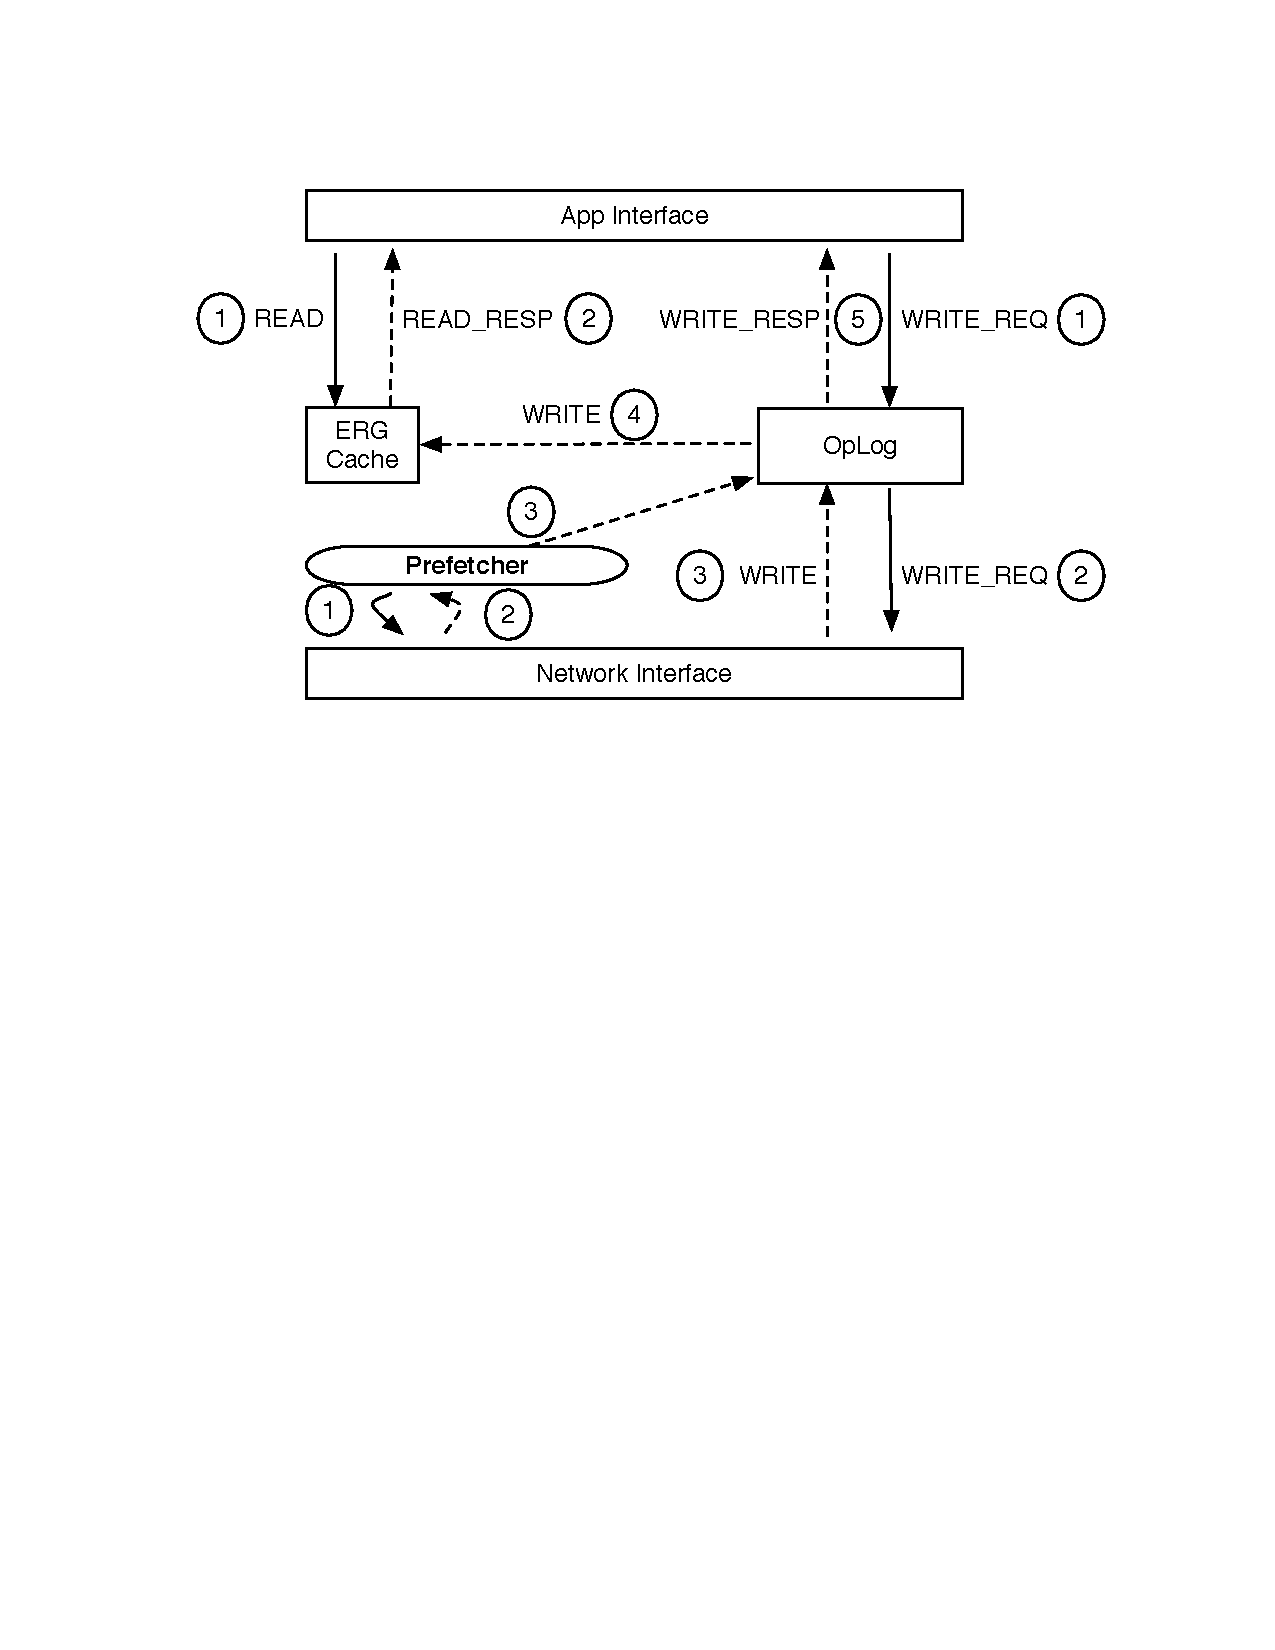
\includegraphics[scale=0.50]{figs/standard_interaction}
\caption{Standard mechanisms for consistency management on the phone.  All READ request go to the local
cached version of the ERG.  All WRITES must go through the OpLog.}
\label{fig:basic_arch}
\end{center}
\end{figure}

Figure~\ref{fig:basic_arch} shows a high-level overview of the components in the architecture and how they interact.  We discuss 
these components in the following secions.  We start with the library that runs on the client and the optional library to run
on the server.  We also discuss the benefits and implications of using either just the client or both the client and server
stubs, particularly with respect to the consistency model.


\section{Client stub}

\subsection{API design rationale}
Different mobile applications have different consistency, energy, and responsiveness requirements.  Unlike traditional application, mobile application
need to be able to continuous adjust their approach to fall on different points in the trade-off space along each of these axes,
throughout the lifetime of the application.  Our goal is to design an API where the application programmer can reason about and 
implement applications that dynamically adjust their position along these three tradeoff axes as the runtime conditions change.

% \subsection{Log dump measurements}
\begin{table*}
\begin{center}
  \begin{tabular}{| r | p{9cm}  | }
    \hline
    {\bf API call } & {\bf Description }  \\ \hline
    read(objectName) & Reads the object from the server if a connection is available.  Otherwise, reads from the local cache. \\ \hline
    read(objectName, freshness) & Reads the object from local cache if it's $\leq$ freshness time units old.  Otherwise, reads from server. \\ \hline
    read(objectName, callback) & Reads from the server when the server is available.  Callback is triggered after the fetch is complete. \\ \hline
    write(objectName, data, op) & Sends a request to the server to apply the operation remotely and copies the object locally after the operation complete.  If the server is unavailable, applies the operation locally and logs it. \\ \hline
    write(objectName, data, op, freshness) & Writes the operation to local copy if it is $\leq$ freshness time units.  Otherwise tries to write to the server. \\ \hline
    write(objectName, data, op, callback) & Writes to the server.  Callback is triggered when the write is complete.  A local copy is cached. \\
    \hline
    query(args) & Send the query to the application server.  If the application server is unavailable, attempts execute the query locally. \\ \hline
    query(args, freshness) & Attempts to answer the query locally if all the application objects involved were updated less than freshness time units ago. \\ \hline
    query(args, callback) & Send the query to the server and triggers the given callback when the query returns. \\ \hline
  \end{tabular}
\caption{Summary of the main API calls of the Context Object Layer.  Each call allows the designer to reason about and implement
along different points in the tradeoff space between consistency, responsiveness/availability, and energy consumption.}
\label{tab:api}
\end{center}
\end{table*}

\subsubsection{Consistency}
Eventually consistency is the consistency model that can be reasonably be implemented in our system.  Variable bandwidth and disconnection,
as well as varible energy consumption policies constraint the consistency model to best effort, eventually consistent.  All clients eventually
 see exactly the same sequence of changes of the values for each object.  We draw an important semantic distinction between the use
 of the just the client stub and the client-server combination.  Using only the client stub gives speculative eventual consistency.
 Operations are performed, proactively, on local copies of the object.  At some point in the future, those updates will be applied
 to the server.  If the server cannot execute the given operations, the server object is copied on the server and the application
 is notified.

 Operations are an important components of the approach we take.  We force the application designer to define the set of operations
 that can be performed by the application server, so that they may also be applied on local copies of objects.  For some applications, 
 sets of operations must be performed atomically, or not at all.  We define such a collection as an \emph{Expression}.  Expressions
 are only supported if the server stub is implemented, since only the server can execute operational sets atomically and
 only the server can resolve conflicts between clients.

\subsubsection{Availability and responsiveness}
Network connection availability and quality change through space and time. Most applications need to make in-time decisions about which
data and how much data they are going to fetch for the application.  For indoor, interactive application, the network conditions can
vary substantially in different parts of the indoor environment.  Our api must support a caching layer for responsiveness and
proactive preftching for availability.  We aim to allow the user to vary the size and frequency of the prefetch mechanism, thereby
allowing for dynamic adjustment of application performance and availability as conditions dictate.

\subsubsection{Battery lifetime}
We can attain high levels of consistency at a higher average cost of energy, by making our all writes go directly to the application server.
For each read/write of an application object, there's an associated, time-varying, cost.  Our API should allow applications to make the 
appropriate choice, given the current opertional conditions.  For example, we can achieve high levels of consistency if all reads/writes are
write-through to the server.  At the other end of the spectrum, we do all reads/writes from locally.  In the latter, we run the risk
of dealing with stale objects.

Table~\ref{tab:api} shows the basic API that is made available to the runtime of the client application.  We essentially support three
types of calls, each with three different sets of parameter and their own semantics.


\subsection{Server stub}

\section{Application example: Energy Lens}

\subsection {Access pattern and available}

\subsection {Uptime distribution}



